\chapter{Plastik dan Bahan Sintetis}\label{ch:g8:plastics}

Hitunglah benda \omterm{def:g8:plastics:plastic}{plastik} yang kamu sentuh dalam satu pagi: sikat gigi,
botol, jas hujan, sarung ponsel, kursi bus, dan kantong belanja. Hampir tak
satu pun di antaranya ada seratus dua puluh tahun yang lalu, dan tak
satu pun tumbuh di pohon atau digali dari dalam tanah. \omterm{def:g8:plastics:plastic}{Plastik} adalah
bahan yang ditemukan para ahli kimia --- ringan, murah, kedap air, dapat
dibentuk menjadi apa saja --- dan justru keberhasilan itu telah menjadi
masalah.

\begin{recall}
\omterm{def:g5:raw-materials-and-recycling:natural-material}{Bahan alami} dipakai hampir seperti ketika ditemukan di alam; \omterm{def:g5:raw-materials-and-recycling:natural-material}{bahan
buatan} dibuat dari \omterm{def:g5:raw-materials-and-recycling:raw-material}{bahan baku} dengan mengubahnya, dan \omterm{def:g5:raw-materials-and-recycling:recycling}{daur ulang}
mengubah bahan benda-benda lama menjadi benda baru
(\cref{ch:g5:raw-materials-and-recycling}). \omterm{def:g4:what-a-fire-needs:burning}{Pembakaran} \omterm{def:g4:what-a-fire-needs:fuel}{bahan bakar} yang
terdiri atas karbon dan hidrogen menghasilkan karbon dioksida dan air
(\cref{ch:g8:combustion-and-fuels}).
\end{recall}

\begin{omfigure}
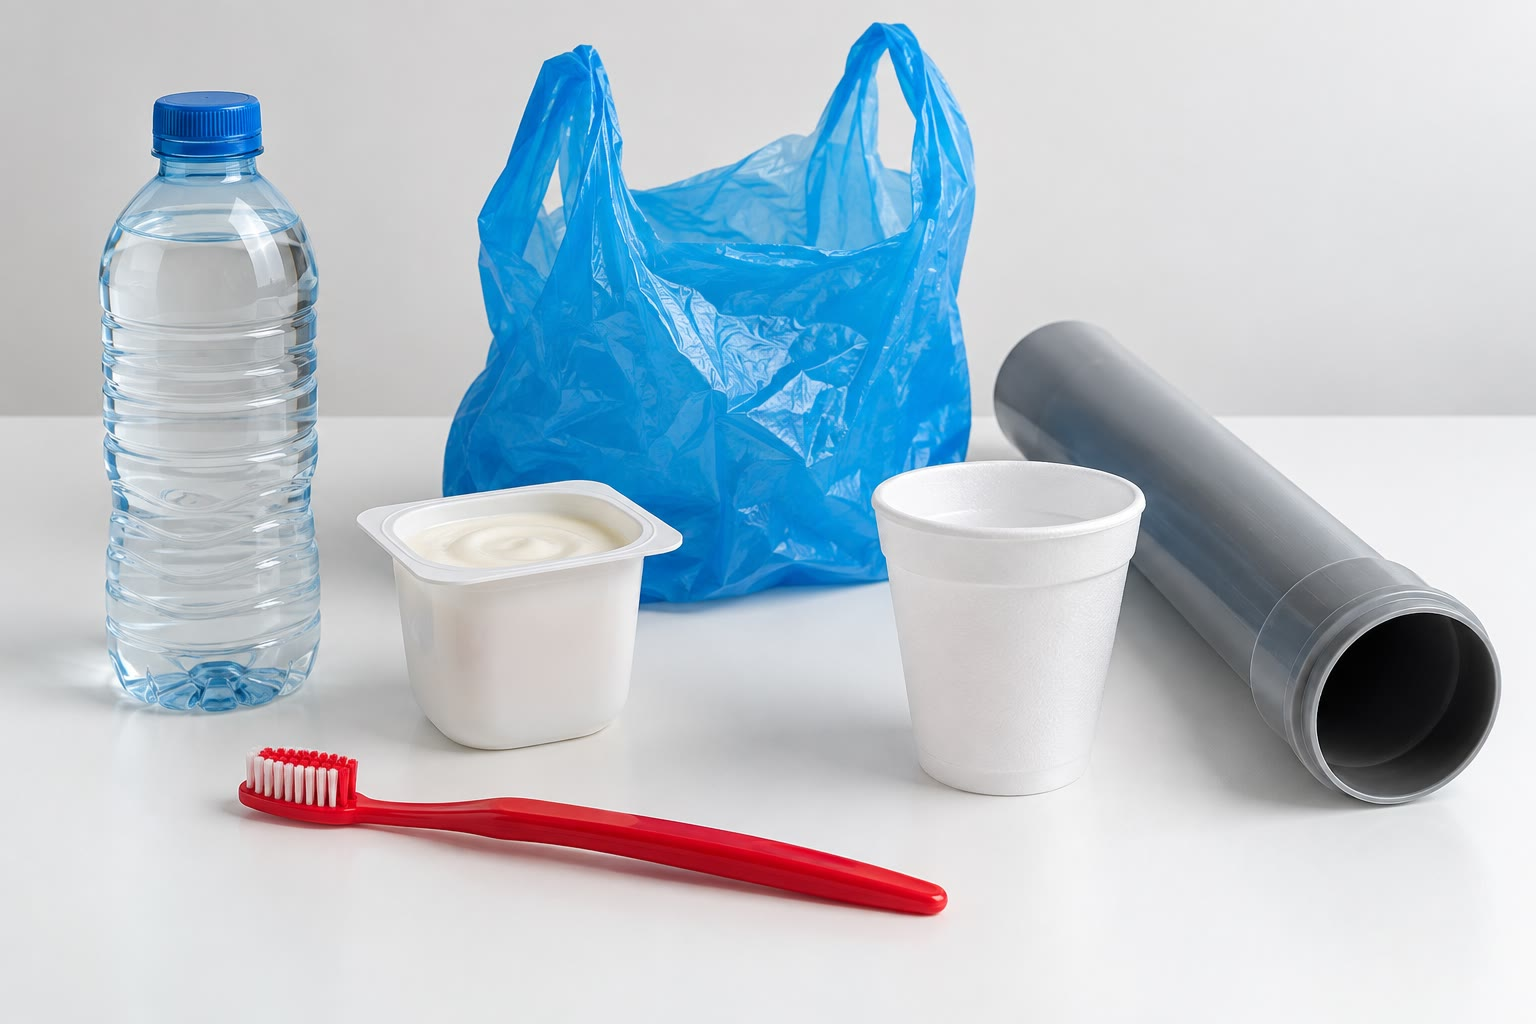
\includegraphics[width=0.55\linewidth]{images/book1/ai/g8-plastic-objects.jpg}

{\small Benda \omterm{def:g8:plastics:plastic}{plastik} sehari-hari: botol, pot, kantong, pipa, cangkir,
sikat gigi.}
\end{omfigure}

\section{Bahan alami, artifisial, dan sintetis}

\begin{definition}[Bahan artifisial dan bahan sintetis]\label{def:g8:plastics:artificial}
Di antara \omterm{def:g5:raw-materials-and-recycling:natural-material}{bahan buatan}, sebuah \emph{bahan
artifisial}\index{bahan artifisial} dibuat dengan mengubah secara kimia
sebuah \omterm{def:g5:raw-materials-and-recycling:natural-material}{bahan alami}: kertas dan viskosa (sejenis kain) dari selulosa
kayu. Sebuah \emph{bahan sintetis}\index{bahan sintetis} dibuat dari
zat-zat yang dibangun para ahli kimia, paling sering dari minyak bumi,
dan tidak memiliki padanan alami: nilon, poliester, \omterm{def:g8:plastics:plastic}{plastik}.
\end{definition}

\begin{omfigure}
\begin{tikzpicture}[font=\small, level distance=1.5cm,
    box/.style={draw=omDef, fill=omDef!6, rounded corners=2pt, align=center,
      inner sep=4pt, text width=3.3cm},
    level 1/.style={sibling distance=6.4cm},
    level 2/.style={sibling distance=3.8cm},
    edge from parent/.style={draw, thick, omDef, ->}]
  \node[box] {bahan}
    child {node[box] {alami\\ \footnotesize katun, wol, kayu}}
    child {node[box] {buatan}
      child {node[box] {artifisial\\ \footnotesize kertas, viskosa}}
      child {node[box, draw=omProp, fill=omProp!6] {sintetis\\ \footnotesize nilon,
        poliester, plastik}}};
\end{tikzpicture}

{\small \omterm{def:g5:raw-materials-and-recycling:natural-material}{Bahan alami}, artifisial, dan sintetis.}
\end{omfigure}

\section{Apa itu plastik}

\begin{definition}[Plastik]\label{def:g8:plastics:plastic}
Yang disebut \emph{plastik}\index{plastik} adalah \omterm{def:g8:plastics:artificial}{bahan sintetis} yang
tersusun atas \omterm{def:g7:atoms-and-molecules:molecule}{molekul-molekul} yang sangat panjang, yang dapat dibentuk
dengan pencetakan --- paling sering selagi panas dan lunak --- dan
mempertahankan bentuknya setelah dingin. Kebanyakan plastik dibuat dari
minyak bumi atau gas alam.
\end{definition}

\begin{remark}[Molekul yang sangat panjang]\label{rem:g8:plastics:long}
Satu \omterm{def:g7:atoms-and-molecules:molecule}{molekul} air mengandung tiga \omterm{def:g7:atoms-and-molecules:atom}{atom}; satu \omterm{def:g7:atoms-and-molecules:molecule}{molekul} \omterm{def:g8:plastics:plastic}{plastik} dapat
mengandung puluhan ribu \omterm{def:g7:atoms-and-molecules:atom}{atom}, yang tergabung dalam rantai panjang,
seperti kalung dari manik-manik yang identik. Cara membangun rantai
seperti itu menjadi pokok bahasan sebuah bab di akhir buku ini.
\end{remark}

\begin{omfigure}
\begin{tikzpicture}[font=\small]
  \foreach \k in {0,...,17} {
    \pgfmathsetmacro\x{0.62*\k}
    \pgfmathsetmacro\y{0.35*sin(40*\k)}
    \shade[ball color=omDef!50] (\x,\y) circle (0.22);
  }
  \node[anchor=west] at (11.2,0) {\dots};
  \node[anchor=north, align=center] at (5.3,-0.6) {rantai dari ribuan satuan yang identik};
\end{tikzpicture}

{\small Sebuah gambaran, bukan model: \omterm{def:g7:atoms-and-molecules:molecule}{molekul} \omterm{def:g8:plastics:plastic}{plastik} adalah rantai
yang sangat panjang dari satuan-satuan yang identik.}
\end{omfigure}

\begin{history}[Bakelit, 1907]
\omterm{def:g8:plastics:plastic}{Plastik} sintetis sepenuhnya yang pertama dibuat oleh ahli kimia Leo
Baekeland pada tahun 1907, dari fenol, yang diperoleh dari ter batu
bara, dan formaldehida. Bakelit, yang keras, gelap, dan tahan panas,
menjadi bahan telepon, radio, dan sakelar listrik. Nilon menyusul pada
tahun 1930-an, lalu \omterm{def:g8:plastics:plastic}{plastik} untuk botol dan kantong sesudah Perang
Dunia Kedua.
\end{history}

\begin{omfigure}
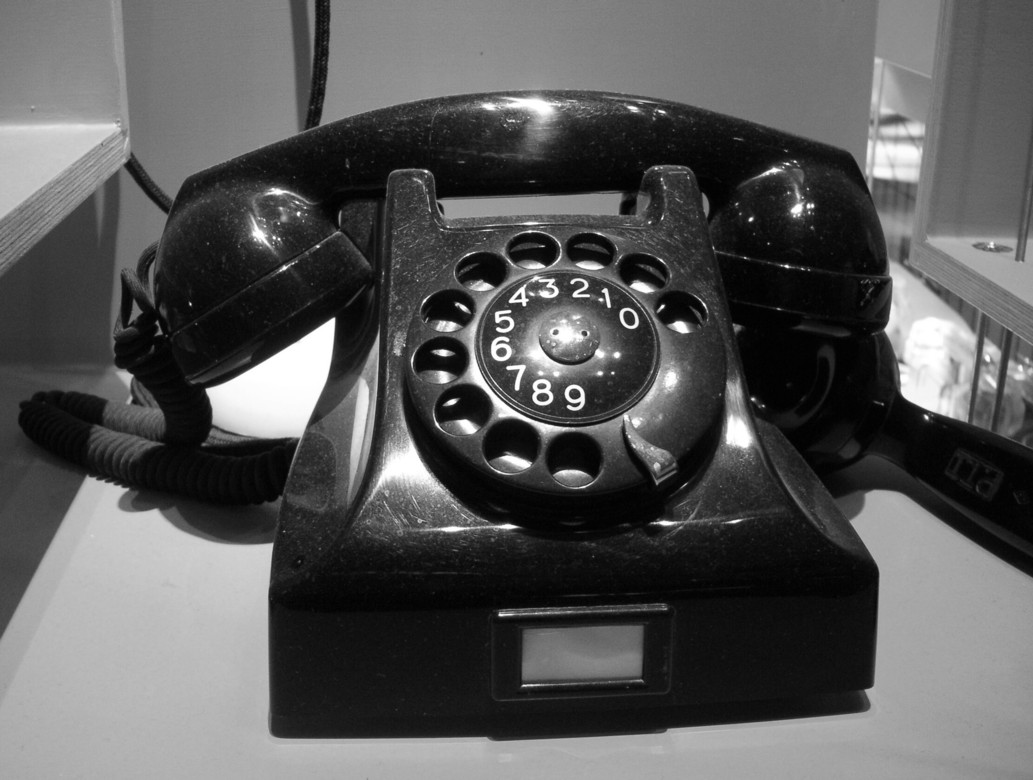
\includegraphics[width=0.42\linewidth]{images/book1/bakelite-telephone.jpg}

{\small Telepon Bakelit tahun 1947. Foto: Holger Ellgaard,
CC\ BY-SA\ 3.0.}
\end{omfigure}

\section{Plastik-plastik utama dan kodenya}

\begin{definition}[Kode identifikasi resin]\label{def:g8:plastics:code}
Yang disebut \emph{kode identifikasi resin}\index{kode identifikasi resin}
adalah sebuah angka dari 1 sampai 7, yang dicetak di dalam segitiga
anak panah pada benda \omterm{def:g8:plastics:plastic}{plastik}, yang menyebutkan \omterm{def:g8:plastics:plastic}{plastik} bahannya,
sehingga benda itu dapat dipilah untuk didaur ulang. Segitiga itu tidak
berarti bahwa benda itu akan didaur ulang.
\end{definition}

\begin{proposition}[Tujuh kode]\label{prop:g8:plastics:codes}
Kode-kode itu, beserta kegunaan yang paling umum dari setiap \omterm{def:g8:plastics:plastic}{plastik}:
\begin{center}
\small
\begin{tabular}{cll}
\hline
kode & \omterm{def:g8:plastics:plastic}{plastik} & benda yang khas \\
\hline
1 & PET, polietilena tereftalat & botol air dan minuman soda, serat kain bulu sintetis \\
2 & HDPE, polietilena densitas tinggi & botol susu dan sampo, tutup botol \\
3 & PVC, polivinil klorida & pipa, kusen jendela, kabel \\
4 & LDPE, polietilena densitas rendah & kantong, lembaran film \\
5 & PP, polipropilena & wadah yoghurt, tutup botol, bemper mobil \\
6 & PS, polistirena & gelas dan nampan busa, wadah CD \\
7 & \omterm{def:g8:plastics:plastic}{plastik} lain & \omterm{def:g6:pure-substances-and-mixtures:mixture}{campuran}, kemasan berlapis-lapis \\
\hline
\end{tabular}
\end{center}
\end{proposition}

\begin{omfigure}
\begin{tikzpicture}[font=\small]
  \foreach \n/\lab in {1/PET, 2/HDPE, 3/PVC, 4/LDPE, 5/PP, 6/PS, 7/LAINNYA} {
    \begin{scope}[xshift=(\n-1)*2.1cm]
      \foreach \a in {90,210,330} {
        \pgfmathsetmacro\b{\a+120}
        \draw[omDef, line width=1.1pt, ->, >={Stealth[length=4pt]}]
          ($(\a:0.75)!0.14!(\b:0.75)$) -- ($(\a:0.75)!0.86!(\b:0.75)$);
      }
      \node[font=\bfseries] at (0,-0.05) {\n};
      \node[anchor=north, font=\footnotesize] at (0,-0.8) {\lab};
    \end{scope}
  }
\end{tikzpicture}

{\small Ketujuh \omterm{def:g8:plastics:code}{kode identifikasi resin}, masing-masing dengan nama
singkat \omterm{def:g8:plastics:plastic}{plastiknya}.}
\end{omfigure}

\section{Termoplastik dan termoset}

\begin{definition}[Termoplastik dan termoset]\label{def:g8:plastics:thermoplastic}
Sebuah \emph{termoplastik}\index{termoplastik} melunak setiap kali
dipanaskan dan mengeras lagi ketika mendingin: termoplastik dapat
dilelehkan dan dicetak lagi berulang-ulang (PET, polietilena, PVC,
polipropilena, polistirena). Sebuah \emph{termoset}\index{termoset}
mengeras untuk selamanya ketika pertama kali dipanaskan dan dicetak:
jika dipanaskan lagi, termoset tidak melunak tetapi menghangus (Bakelit,
resin pada lem dan pada lambung perahu).
\end{definition}

\begin{remark}[Yang dapat didaur ulang]\label{rem:g8:plastics:which}
\omterm{def:g8:plastics:thermoplastic}{Termoplastik} dapat dilelehkan dan dicetak ulang: itulah \omterm{def:g8:plastics:plastic}{plastik} yang
didaur ulang menjadi benda baru. \omterm{def:g8:plastics:thermoplastic}{Termoset} tidak dapat dilelehkan lagi.
\end{remark}

\section{Plastik di lingkungan}

\begin{proposition}[Plastik itu awet]\label{prop:g8:plastics:last}
% ledger: plastics:use-2019, plastics:waste-2019, plastics:recycled-share-2019
Dunia memakai sekitar 460 juta ton \omterm{def:g8:plastics:plastic}{plastik} pada tahun 2019 dan membuang
sekitar 353 juta ton sampah \omterm{def:g8:plastics:plastic}{plastik}; \omterm{def:g8:plastics:plastic}{plastik} \omterm{def:g5:raw-materials-and-recycling:recycling}{daur ulang} hanya sekitar
\qty{6}{\percent} dari \omterm{def:g8:plastics:plastic}{plastik} yang dipakai. \omterm{def:g8:plastics:plastic}{Plastik} tidak membusuk: di
alam, \omterm{def:g8:plastics:plastic}{plastik} pecah menjadi kepingan yang makin lama makin kecil, yaitu
mikroplastik, yang ditemukan di sungai, samudra, tanah, dan tubuh
hewan.
\end{proposition}

\begin{omfigure}
\begin{minipage}[t]{0.48\linewidth}\centering
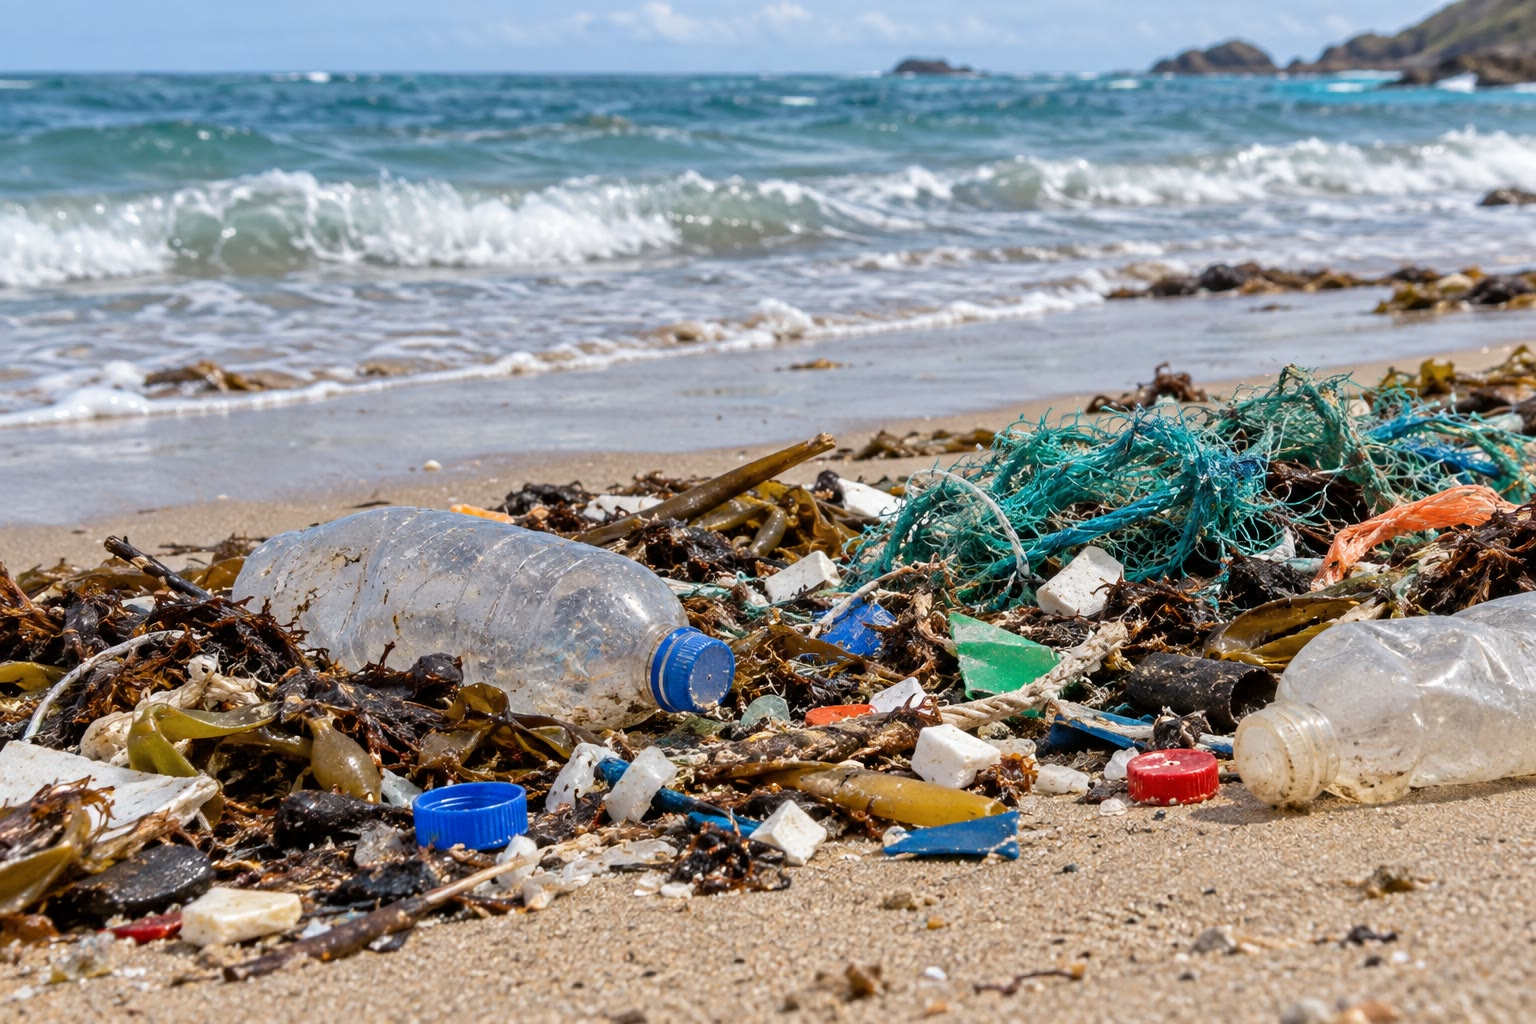
\includegraphics[width=\linewidth,height=4.6cm,keepaspectratio]{images/book1/ai/g8-beach-litter.jpg}

{\small Sampah \omterm{def:g8:plastics:plastic}{plastik} yang terdampar di pantai.}
\end{minipage}\hfill
\begin{minipage}[t]{0.48\linewidth}\centering
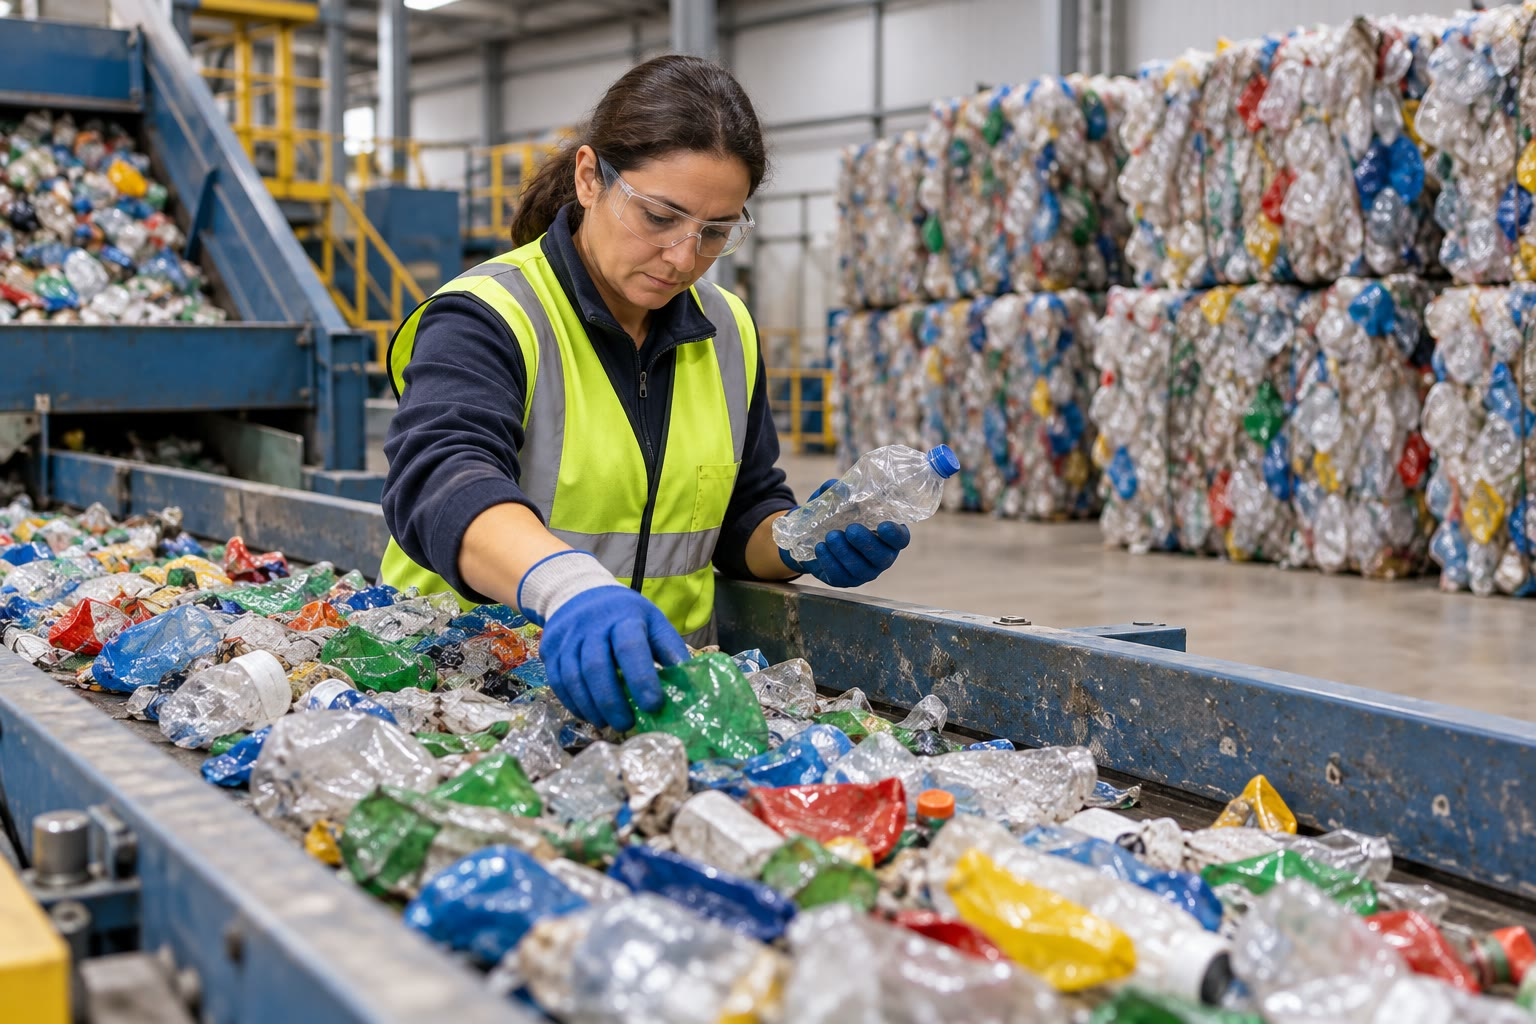
\includegraphics[width=\linewidth,height=4.6cm,keepaspectratio]{images/book1/ai/g8-sorting-line.jpg}

{\small Jalur pemilahan di pabrik \omterm{def:g5:raw-materials-and-recycling:recycling}{daur ulang} \omterm{def:g8:plastics:plastic}{plastik}.}
\end{minipage}
\end{omfigure}

\begin{remark}[Membakar plastik]\label{rem:g8:plastics:burning}
\omterm{def:g8:plastics:plastic}{Plastik} dapat \omterm{def:g4:what-a-fire-needs:burning}{terbakar}, dan menghasilkan karbon dioksida jika \omterm{def:g4:what-a-fire-needs:burning}{terbakar}
sempurna. Tetapi jika dibakar di api \omterm{def:g4:what-a-fire-needs:burning}{pembakaran} sampah di halaman,
\omterm{def:g8:plastics:plastic}{plastik} \omterm{def:g4:what-a-fire-needs:burning}{terbakar} tidak sempurna dan melepaskan jelaga, karbon
monoksida, dan zat-zat berbahaya lainnya; PVC, yang mengandung klorin,
melepaskan hidrogen klorida, gas yang korosif. Sampah \omterm{def:g8:plastics:plastic}{plastik} hanya
dibakar di insinerator yang dibangun untuk membersihkan asapnya.
\end{remark}

\section{Latihan}

\begin{exercise}[$\star$]\label{exo:g8:plastics:1}
Alami, artifisial, atau sintetis? Katun, nilon, kertas, wol,
polistirena, viskosa.
\end{exercise}

\begin{exercise}[$\star$]\label{exo:g8:plastics:2}
Dari \omterm{def:g5:raw-materials-and-recycling:raw-material}{bahan baku} apa kebanyakan \omterm{def:g8:plastics:plastic}{plastik} dibuat?
\end{exercise}

\begin{exercise}[$\star$]\label{exo:g8:plastics:3}
\omterm{def:g8:plastics:plastic}{Plastik} apa yang memiliki kode 1? Sebutkan satu benda yang terbuat
darinya.
\end{exercise}

\begin{exercise}[$\star$]\label{exo:g8:plastics:4}
Apa perbedaan antara \omterm{def:g8:plastics:thermoplastic}{termoplastik} dan \omterm{def:g8:plastics:thermoplastic}{termoset}?
\end{exercise}

\begin{exercise}[$\star\star$]\label{exo:g8:plastics:5}
Sebuah wadah yoghurt memuat kode 5. Sebutkan \omterm{def:g8:plastics:plastic}{plastiknya}, dan katakan
apakah wadah itu pada prinsipnya dapat dilelehkan dan dicetak ulang.
\end{exercise}

\begin{exercise}[$\star\star$]\label{exo:g8:plastics:6}
Mengapa segitiga anak panah pada sebuah benda tidak berarti bahwa benda
itu akan didaur ulang?
\end{exercise}

\begin{exercise}[$\star\star$]\label{exo:g8:plastics:7}
Mengapa gagang wajan sering dibuat dari \omterm{def:g8:plastics:thermoplastic}{termoset} dan bukan dari
\omterm{def:g8:plastics:thermoplastic}{termoplastik}?
\end{exercise}

\begin{exercise}[$\star\star$]\label{exo:g8:plastics:8}
Dengan angka-angka tahun 2019 dalam bab ini, berapa persen \omterm{def:g8:plastics:plastic}{plastik} yang
dipakai menjadi sampah pada tahun itu? Bulatkan ke bilangan bulat
terdekat.
\end{exercise}

\begin{exercise}[$\star\star$]\label{exo:g8:plastics:9}
Mengapa PVC tidak boleh dibakar di api \omterm{def:g4:what-a-fire-needs:burning}{pembakaran} sampah di halaman?
\end{exercise}

\begin{exercise}[$\star\star$]\label{exo:g8:plastics:10}
Sebuah sekolah memakai 300 botol, masing-masing \qty{25}{g}, setiap
minggu, selama 36 minggu dalam setahun. Berapa massa \omterm{def:g8:plastics:plastic}{plastik} itu dalam
setahun?
\end{exercise}

\begin{exercise}[$\star\star\star$]\label{exo:g8:plastics:11}
Polietilena hanya tersusun atas karbon dan hidrogen. Tuliskan produk
\omterm{def:g8:combustion-and-fuels:complete}{pembakaran sempurnanya}. Jelaskan mengapa membakarnya menambah karbon
dioksida ke \omterm{def:g4:air-a-mixture-of-gases:air}{udara} seperti \omterm{def:g8:combustion-and-fuels:fossil}{bahan bakar fosil}.
\end{exercise}

\begin{exercise}[$\star\star\star$]\label{exo:g8:plastics:12}
Jelaskan bagaimana botol \omterm{def:g8:plastics:plastic}{plastik} yang hilang di laut dapat berakhir,
bertahun-tahun kemudian, sebagai mikroplastik di dalam tubuh ikan.
\end{exercise}

\section{Soal: Jalur Pemilahan}

\begin{problem}[{Soal akhir pekan --- satu ton botol bekas, kodenya, dan
serpihan plastik bersih yang keluar dari pabrik}]
\label{pb:g8:plastics:1}
Sebuah pabrik \omterm{def:g5:raw-materials-and-recycling:recycling}{daur ulang} menerima bongkahan botol minuman bekas.
Sebongkah yang khas seberat \qty{1}{t} (\qty{1000}{kg}) berisi, menurut
massa: \qty{80}{\percent} badan botol dari PET, \qty{12}{\percent} tutup
botol (HDPE dan PP), \qty{5}{\percent} label (lembaran PP), dan
\qty{3}{\percent} kotoran dan sisa cairan. Mesin-mesin memisahkan tutup
dan label dari badan botol, PET-nya digiling menjadi serpihan, dan
serpihan itu dicuci; pencucian itu menghilangkan \qty{2.5}{\percent}
PET. Serpihan yang bersih dilelehkan dan dipintal menjadi serat jaket
bulu sintetis.

\medskip
\noindent\textbf{Bagian I --- \omterm{def:g8:plastics:plastic}{Plastiknya}.}
\begin{enumerate}
  \item Kode apa yang tercetak pada badan botol? Pada tutupnya?
  \item Apakah \omterm{def:g8:plastics:plastic}{plastik-plastik} ini alami, artifisial, atau sintetis?
  \item Dapatkah PET dilelehkan dan dipintal lagi? Jenis \omterm{def:g8:plastics:plastic}{plastik} apakah
        PET jadinya?
  \item Mengapa tutup dan label dipisahkan dari badan botol sebelum
        PET-nya dilelehkan?
\end{enumerate}

\medskip
\noindent\textbf{Bagian II --- Bongkahannya.}
\begin{enumerate}[resume]
  \item Berapa massa PET dalam satu bongkah?
  \item Berapa massa tutup botolnya? Labelnya?
  \item Berapa massa bongkahan yang bukan \omterm{def:g8:plastics:plastic}{plastik}?
  \item Berapa persen bongkahan itu yang berupa \omterm{def:g8:plastics:plastic}{plastik}?
\end{enumerate}

\medskip
\noindent\textbf{Bagian III --- Serpihannya.}
\begin{enumerate}[resume]
  \item Berapa massa PET yang hilang dalam pencucian?
  \item Sebuah jaket bulu sintetis memerlukan \qty{0.39}{kg} serat PET.
        Mengapa lebih baik membuatnya dari serpihan daripada dari PET
        baru?
  \item Pabrik itu dapat saja membakar tutup dan label untuk diambil
        panasnya alih-alih mendaur ulangnya. Sebutkan gas yang akan
        ditambahkannya ke \omterm{def:g4:air-a-mixture-of-gases:air}{udara}.
  \item Hitung massa serpihan PET bersih yang dihasilkan satu bongkah.
\end{enumerate}
\end{problem}
